\section{Transceiver}
\index{transceiver}
\index{sändtagare|see {transceiver}}

\begin{wrapfigure}[26]{R}{0.5\textwidth}
  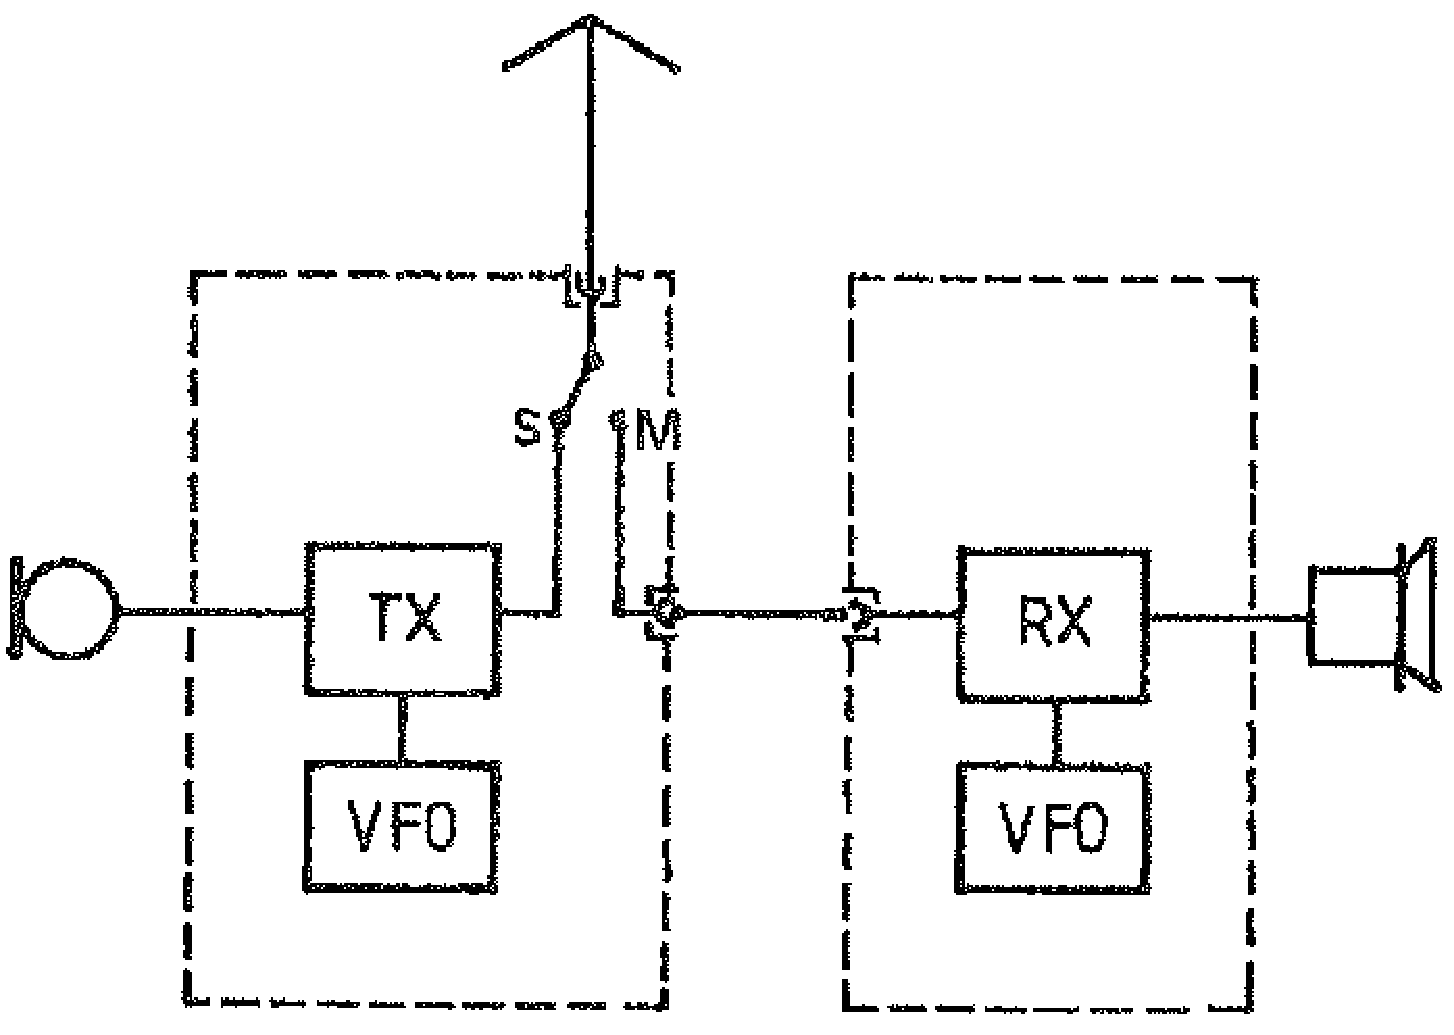
\includegraphics[width=0.5\textwidth]{images/cropped_pdfs/bild_2_5-09.pdf}
  \caption{Separat sändare och mottagare}
  \label{fig:bildII5-9}

  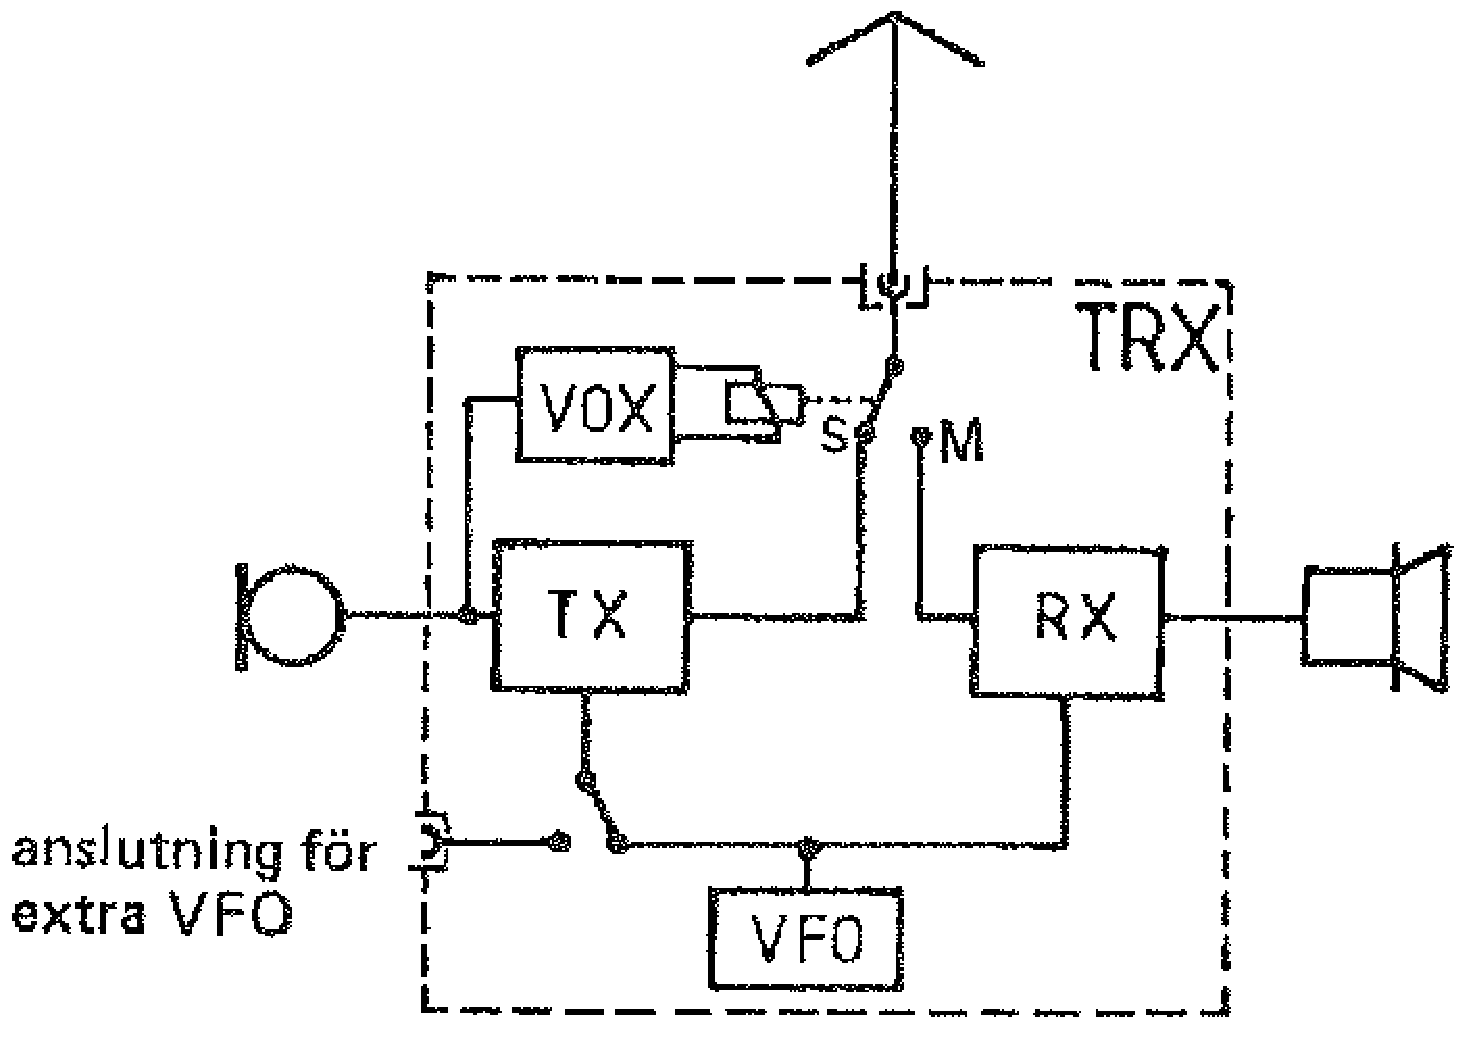
\includegraphics[width=0.5\textwidth]{images/cropped_pdfs/bild_2_5-10.pdf}
  \caption{Transceiver med samma VFO}
  \label{fig:bildII5-10}
\end{wrapfigure}

En \emph{transceiver} -- transmitter receiver -- är både en sändare och
mottagare med delvis gemensamma funktioner.
Dessa kan till exempel vara oscillatorer, signalbehandlingskretsar, filter,
strömförsörjning och så vidare, vilket innebär besparing av ingående
komponenter, men också vissa funktionella begränsningar.

Transceiverkoncept är numera vad som används allra mest av radioamatörer.
Eftersom man på olika vis önskar sig så många sändar- och mottagarfunktioner
som möjligt inom samma skal, så kan det vara svårt att undvika kompromisser.
Så kan till exempel en specialiserad, separat mottagare ha bättre eller fler
egenskaper än i en transceiver.

\subsection{Jämförelse mellan stationskoncept}

Bild \ref{fig:bildII5-9} visar i stort en station med skilda sändar- och
mottagarfunktioner, men att antennen är gemensam.
Bild \ref{fig:bildII5-10} visar i stort en transceiver där VFO och antenn är
gemensamma, men i övrigt med skilda funktioner.
Bild \ref{fig:bildII5-11} visar samma transceiver, men med ett mer detaljerat
blockschema.

\begin{figure}
  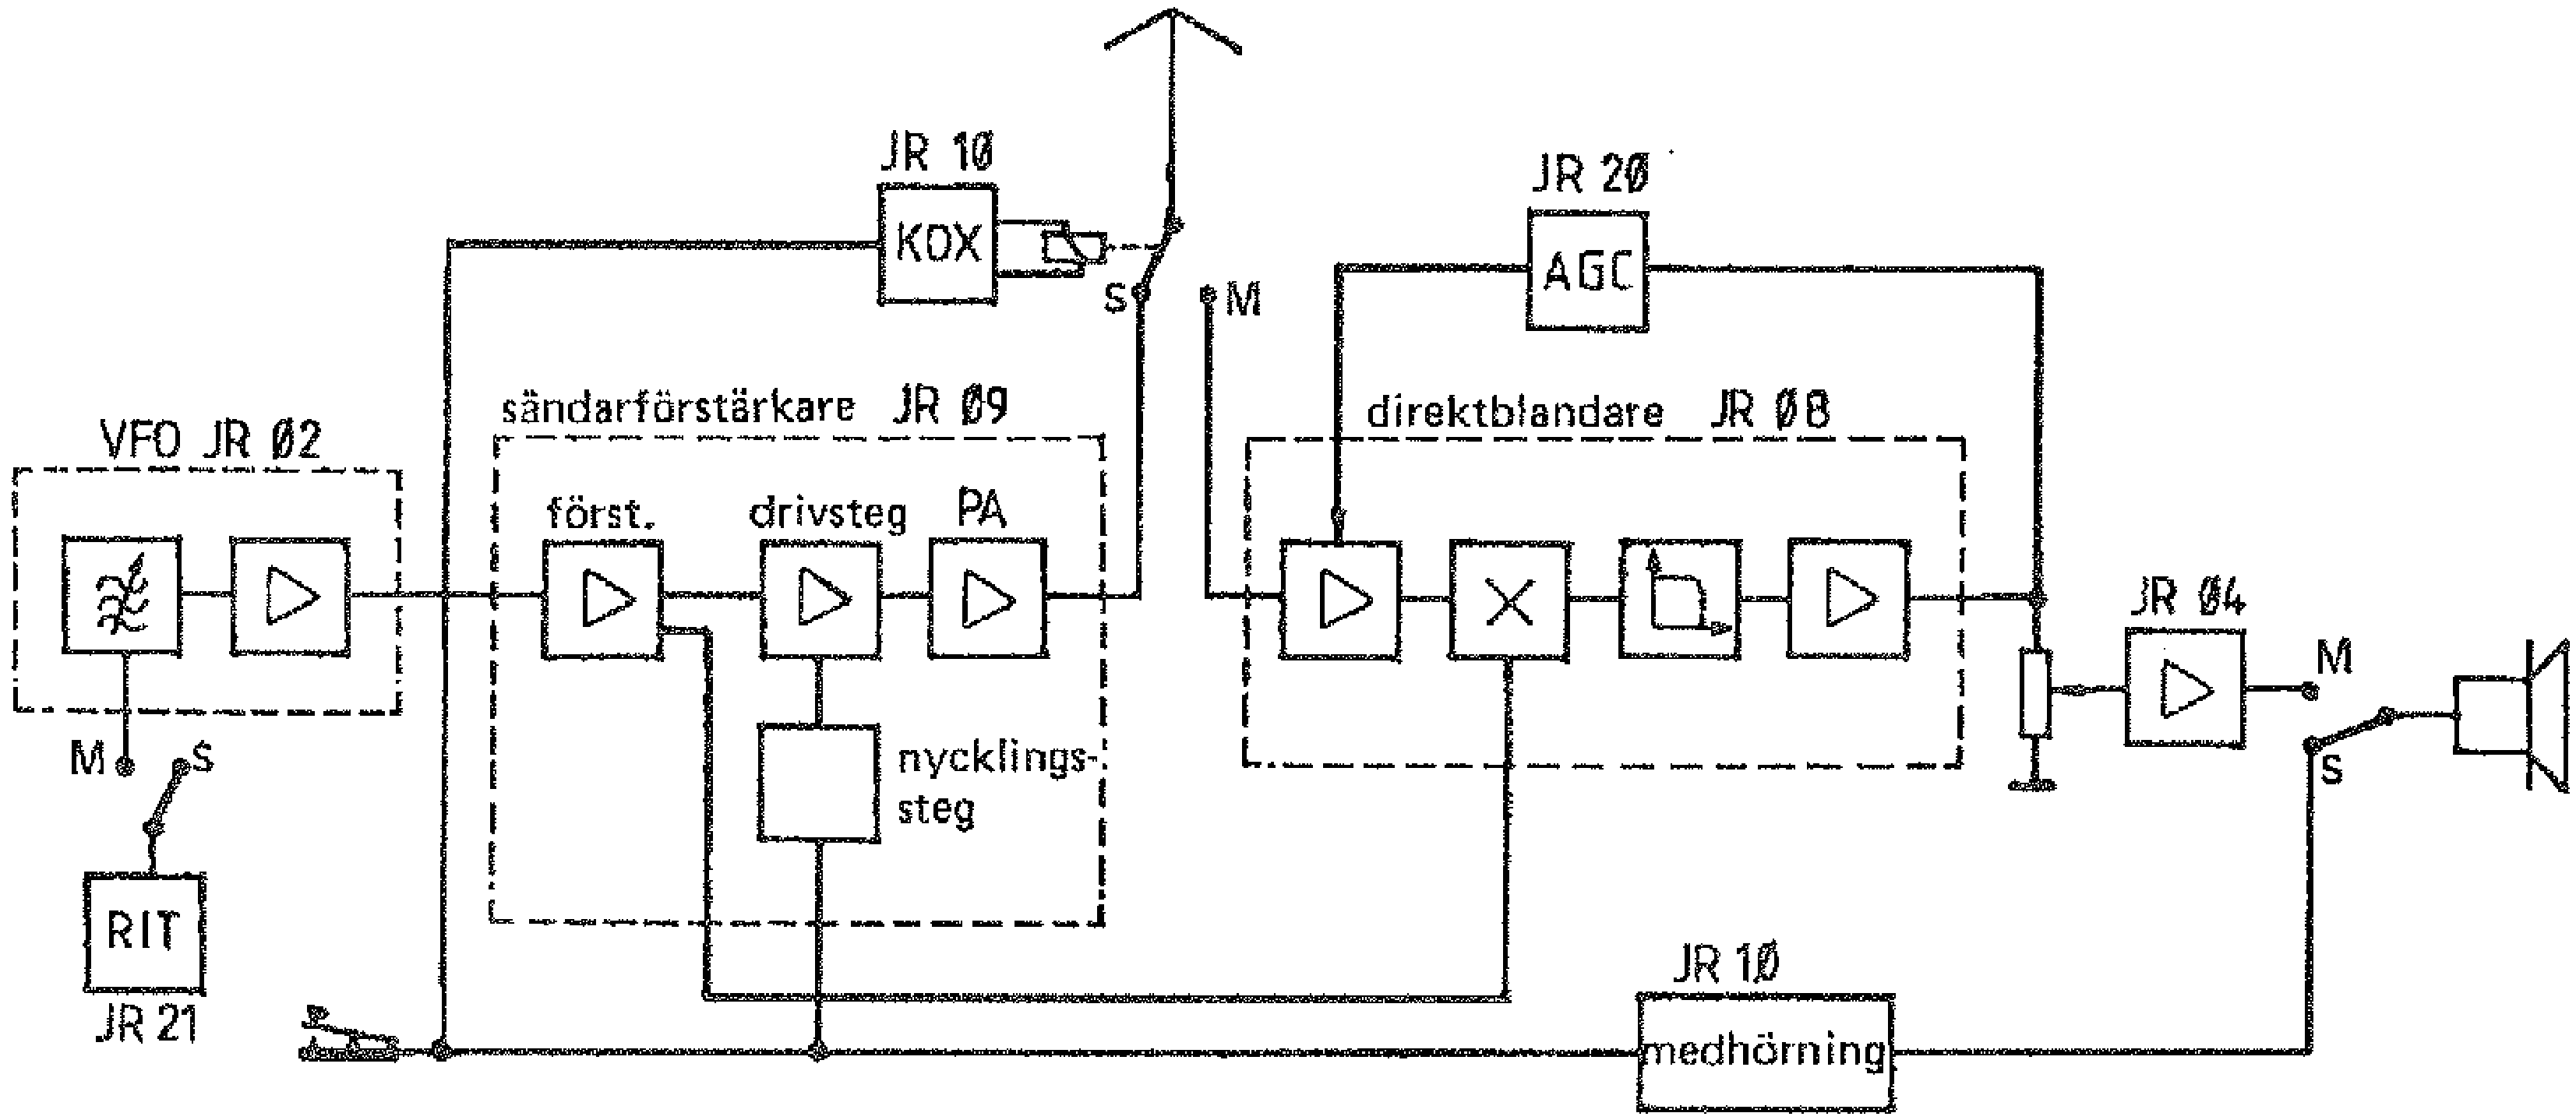
\includegraphics[width=\textwidth]{images/cropped_pdfs/bild_2_5-11.pdf}
  \caption{Direktblandad transceiver med gemensam VFO}
  \label{fig:bildII5-11}
\end{figure}

\subsection{Simplex}
\index{simplex}

En station sägs sända \emph{simplex} när den enbart kan sända eller ta emot,
det vill säga när den inte samtidigt sänder och tar emot.
Detta är det normala för kortvågs-stationer som sänder på samma frekvens.

\subsection{Halv duplex}
\index{halv duplex}
\index{split}

En station sägs sända \emph{halv duplex} (eng. \emph{half duplex}) när den
enbart sänder eller tar emot, det vill säga när den inte samtidigt sänder och
tar emot.
Om detta sker på samma frekvens, så kallas det även simplex, men när stationen
opereras med split frekvens så räcker inte simplex-begreppet men halv duplex
täcker det.

\subsection{Duplex}
\index{full duplex}
\index{duplex}
\index{duplexfilter}
\index{utsläckning}
\index{notch}

En stations sägs sända \emph{duplex} eller \emph{full duplex} när den kan
samtidigt sända och ta emot på två olika frekvenser.

Duplex-operation kräver i allmänhet stor isolation mellan sändare och mottagare,
något som ofta åstadkoms med kavitets-filter kopplade mellan sändare och antenn
och mottagare och antenn.
Om gemensam antenn används, så kopplas dessa kavitetsfilter ihop till vad som
kallas \emph{duplexfilter}.

För en lyckad duplex-operation krävs i allmänhet mer än 100~dB isolation mellan
sändare och mottagare.
Mottagarens kavitetsfilter trimmas så att det får en djup \emph{utsläckning}
(eng. \emph{notch}) vid sändarens frekvens, men med så lite förlust som möjligt
på mottagarens frekvens.
Sändarens kavitetsfilter trimmas så att det får en djup utsläckning/notch vid
mottagarens frekvens, för att på så sätt minimera att sändarens fasbrus höjer
brusgolvet för mottagaren, men med så liten förlust som möjligt på sändarens
frekvens.

\subsection{CW-transceiver med direktblandare}
\index{CW}
\index{transceiver!CW}
\index{direktblandare}
\index{Receiver Incremental Tuning (RIT)}
\index{RIT}
\index{keyed operated xmitter (KOX)}
\index{KOX}

Bild \ref{fig:bildII5-11} visar en enkel transceiver för telegrafi.
Sändaren är en rak sändare och mottagaren arbetar med direktblandning.
För 1-kanaltrafik räcker det med en gemensam VFO för sändning och mottagning.
Om motstationen svarar exakt på sändningsfrekvensen, vilken ju är
VFO-frekvensen, så erhålls svävningsnoll i mottagaren.
För att få hörbara morsetecken är mottagaren utrustad med
\emph{Receiver Incremental Tuning (RIT)}, som ändrar VFO-frekvensen med
cirka 800~Hz vid mottagning.

I konstruktionen finns en anordning kallad \emph{Key Operated Xmitter (KOX)}.
Denna kopplar om transceivern till sändning när telegrafnyckeln trycks ner och
till mottagning igen efter en viss tid sedan nyckeln har släppts upp.
Telegrafnyckeln styr också en tongenerator som ljuder i takt med de sända
morsetecknen, så kallad medhörning.

Denna transceiver är utförd för endast ett frekvensband och i övrigt
mycket enkel.

\subsection{Kristallstyrd FM-transceiver för VHF}
\index{frekvensmodulation}
\index{transceiver!FM}
\index{dubbelsuperheterodyn}

Bild \ref{fig:bildII5-12} visar en kristallstyrd FM-sändare med
frekvensomkopplare för kanalval inom 144--146~MHz-bandet.

En kristallfrekvens av cirka 12~MHz multipliceras 12 gånger i en kedja av
förstärkarsteg för att ge sändningsfrekvensen.
Bilden visar räkneexempel för två frekvenskanaler.
Det frekvenssving i oscillatorn, som alstras av modulatorn,
multipliceras också med 12.
För ett sving av 3~kHz på bärvågen är svinget på oscillatorn bara 250~Hz.

Efter mikrofonförstärkaren följer en amplitudbegränsare, som ska
hålla deviationen inom ett givet maxvärde, oavsett signalstyrkan från
mikrofonen.
Därefter följer ett lågpassfilter, som dels dämpar de övertoner som
uppstår vid amplitudbegränsningen och dels begränsar de höga frekvenserna
i den modulerade signalen.
Båda åtgärderna begränsar bandbredden.

Mottagaren är en \emph{dubbelsuperheterodyn}, ofta kallad för dubbelsuper.
Den mottagna signalen passerar genom ett förselektionsfilter och en
HF-förstärkare för att i 1:a blandaren blandas med en lokal signal.

\begin{figure}
  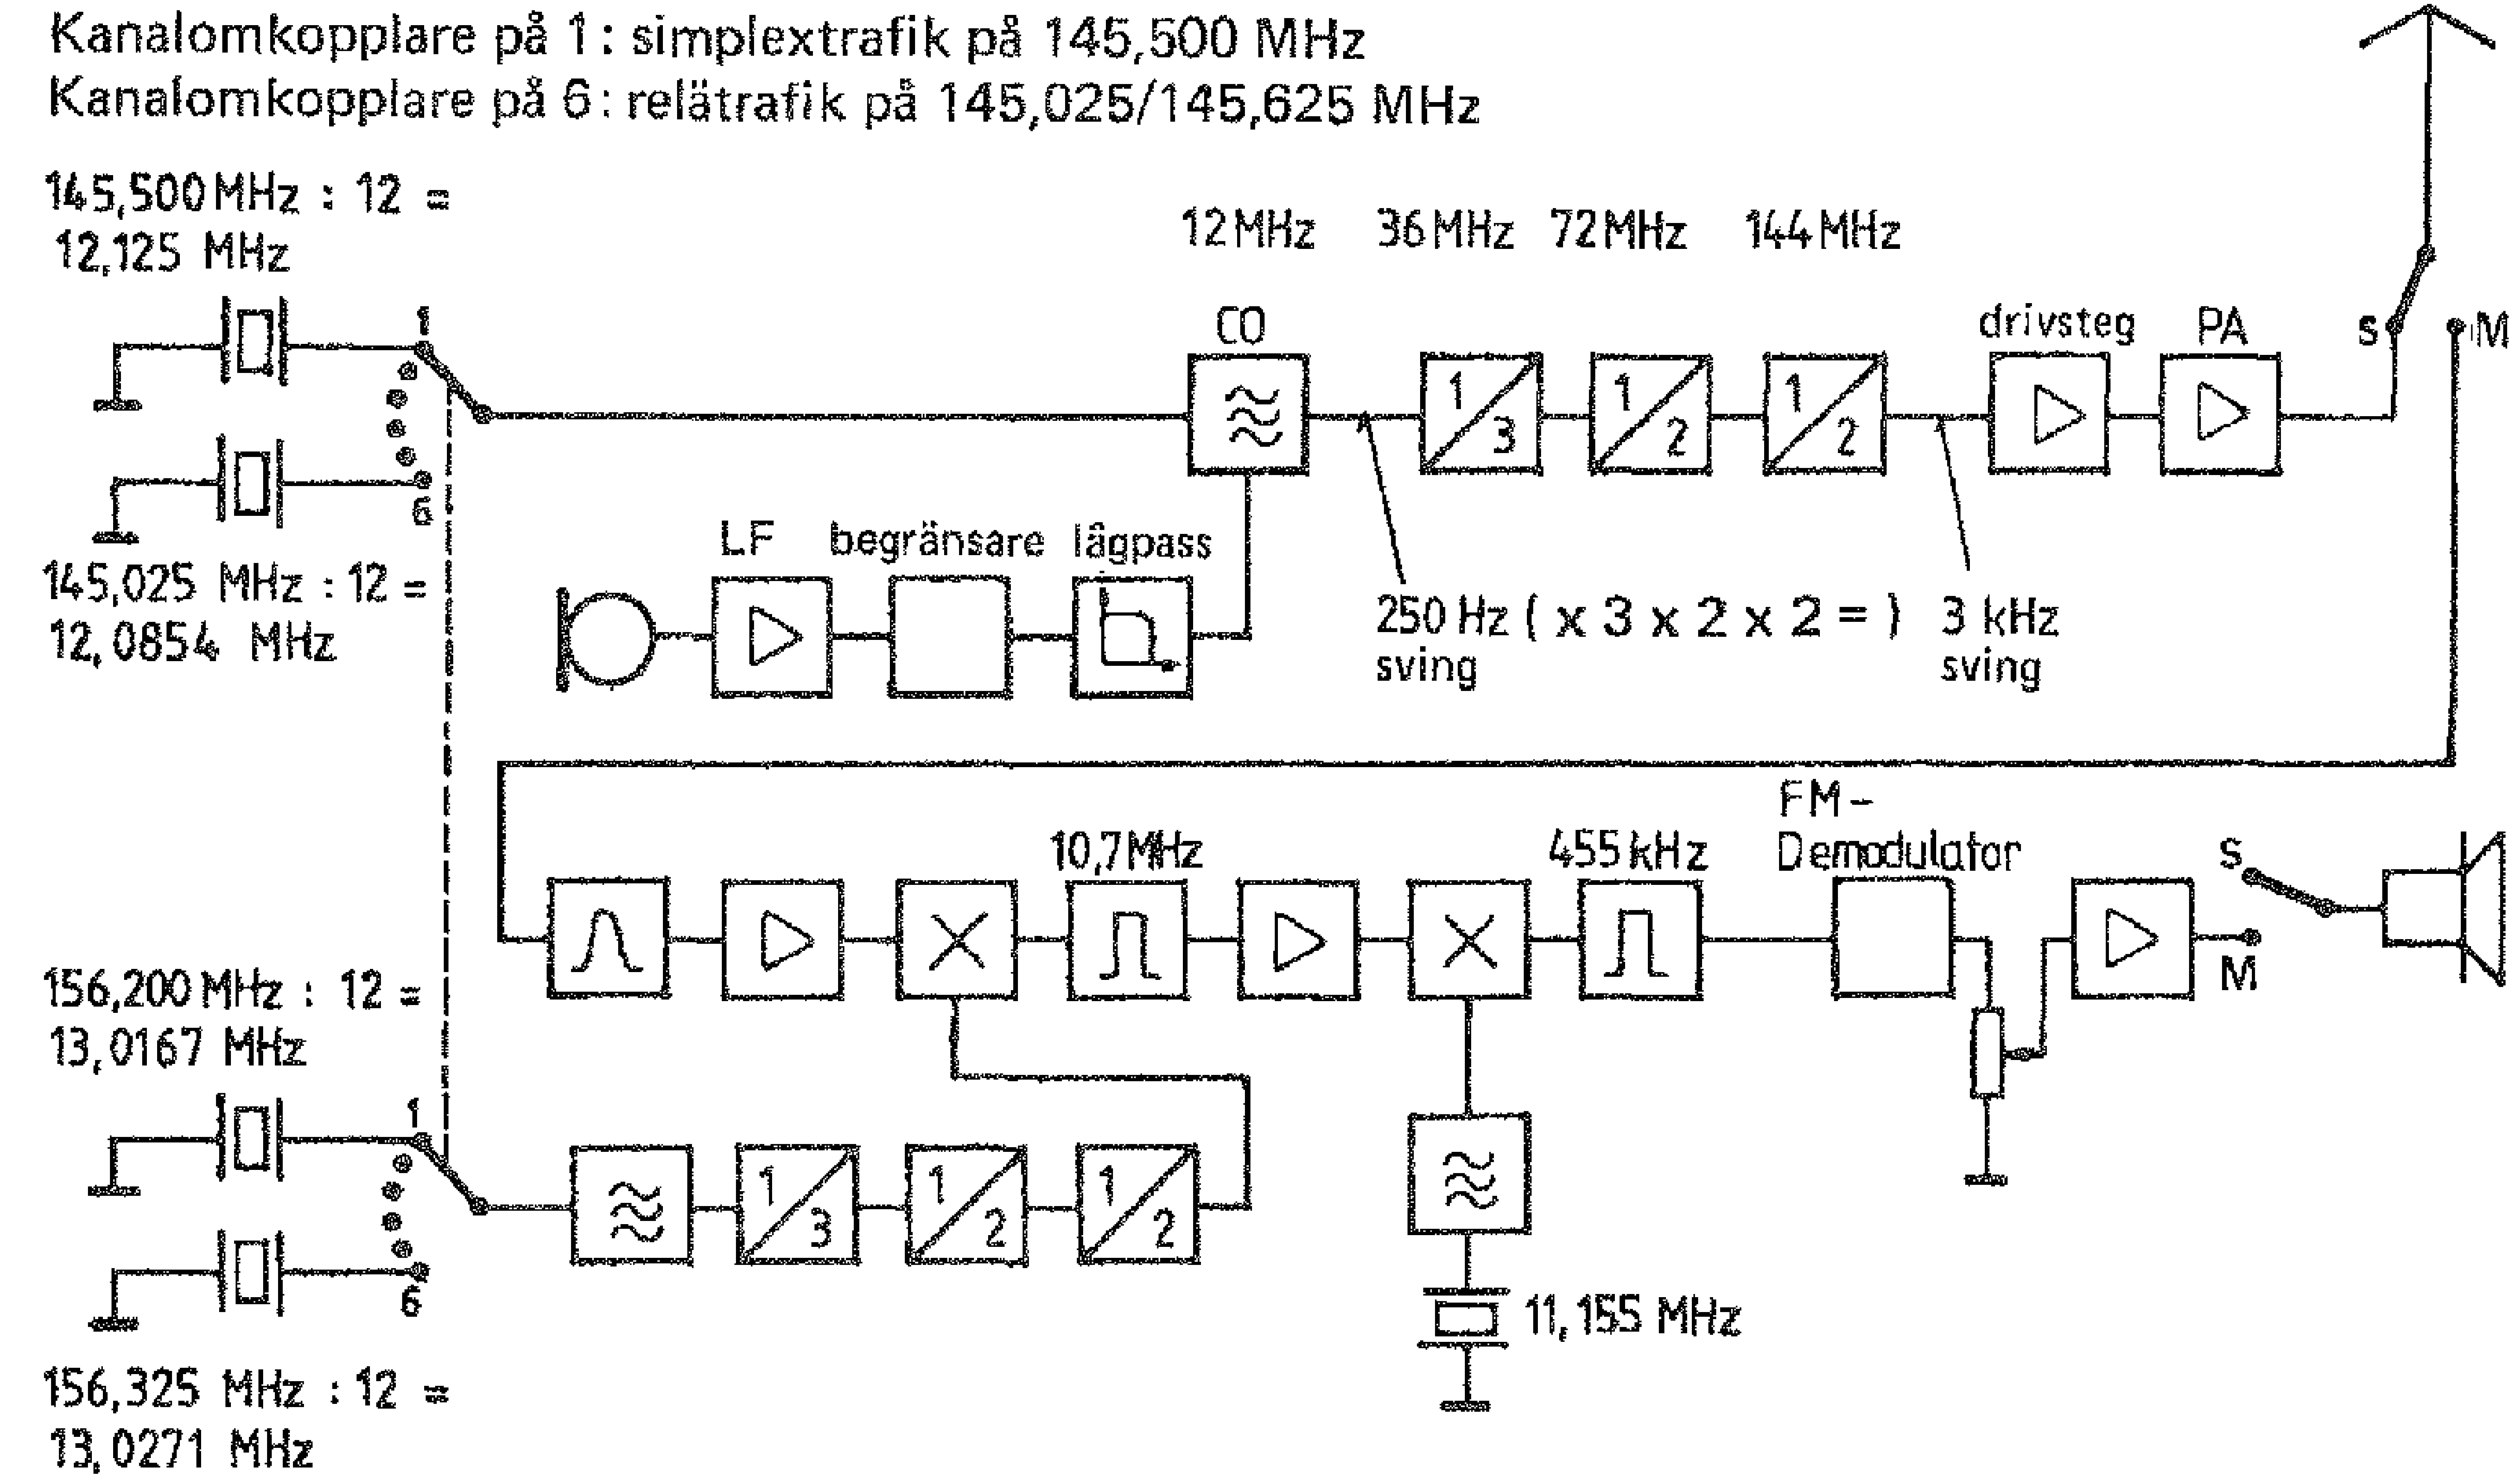
\includegraphics[width=\textwidth]{images/cropped_pdfs/bild_2_5-12.pdf}
  \caption{Kristallstyrd 6-kanals FM-transceiver för VHF}
  \label{fig:bildII5-12}
\end{figure}

%%


En kristallstyrd lokaloscillator med efterföljande
frekvensmultipliceringssteg alstrar denna signal.

Lokaloscillatorkedjans utfrekvens läggs 10,7~MHz över eller under
mottagningsfrekvensen och mellanfrekvensen efter den 1:a blandningen
blir då 10,7~MHz.
Skilda oscillatorer används vid sändning respektive mottagning varför
styrkristallerna för sändning respektive mottagning på en given kanal får
olika frekvens.
Vid omkoppling till en annan kanal väljs ett annat kristallpar, vilket
lämpligen sker med samma omkopplare.

Den relativt höga 1:a mellanfrekvensen 10,7~MHz ger ett så stort
avstånd till spegelfrekvensen, att bandbredden i förselektionsfiltren
är tillräckligt smal för att undertrycka spegelfrekvensen.
Av samma skäl bör 1:a mellanfrekvensen i en UHF-mottagare väljas ytterligare
tre gånger högre.
Den relativt låga 2:a mellanfrekvensen medger en god närselektering
redan med enkla bandfilter.
En eventuell MF-förstärkare ger tillräcklig signalstyrka till FM-demodulatorn.

För denna lösning behövs det två styrkristaller för varje
frekvenskanal, vilket av kostnadsskäl kan vara en nackdel.

\subsection{PLL-styrd FM-transceiver för VHF}
\index{PLL}
\index{frekvensmodulation}
\index{transceiver!PLL}
\index{transceiver!FM}
\index{dubbelsuperheterodyn}
\index{simplex}

\begin{figure}
  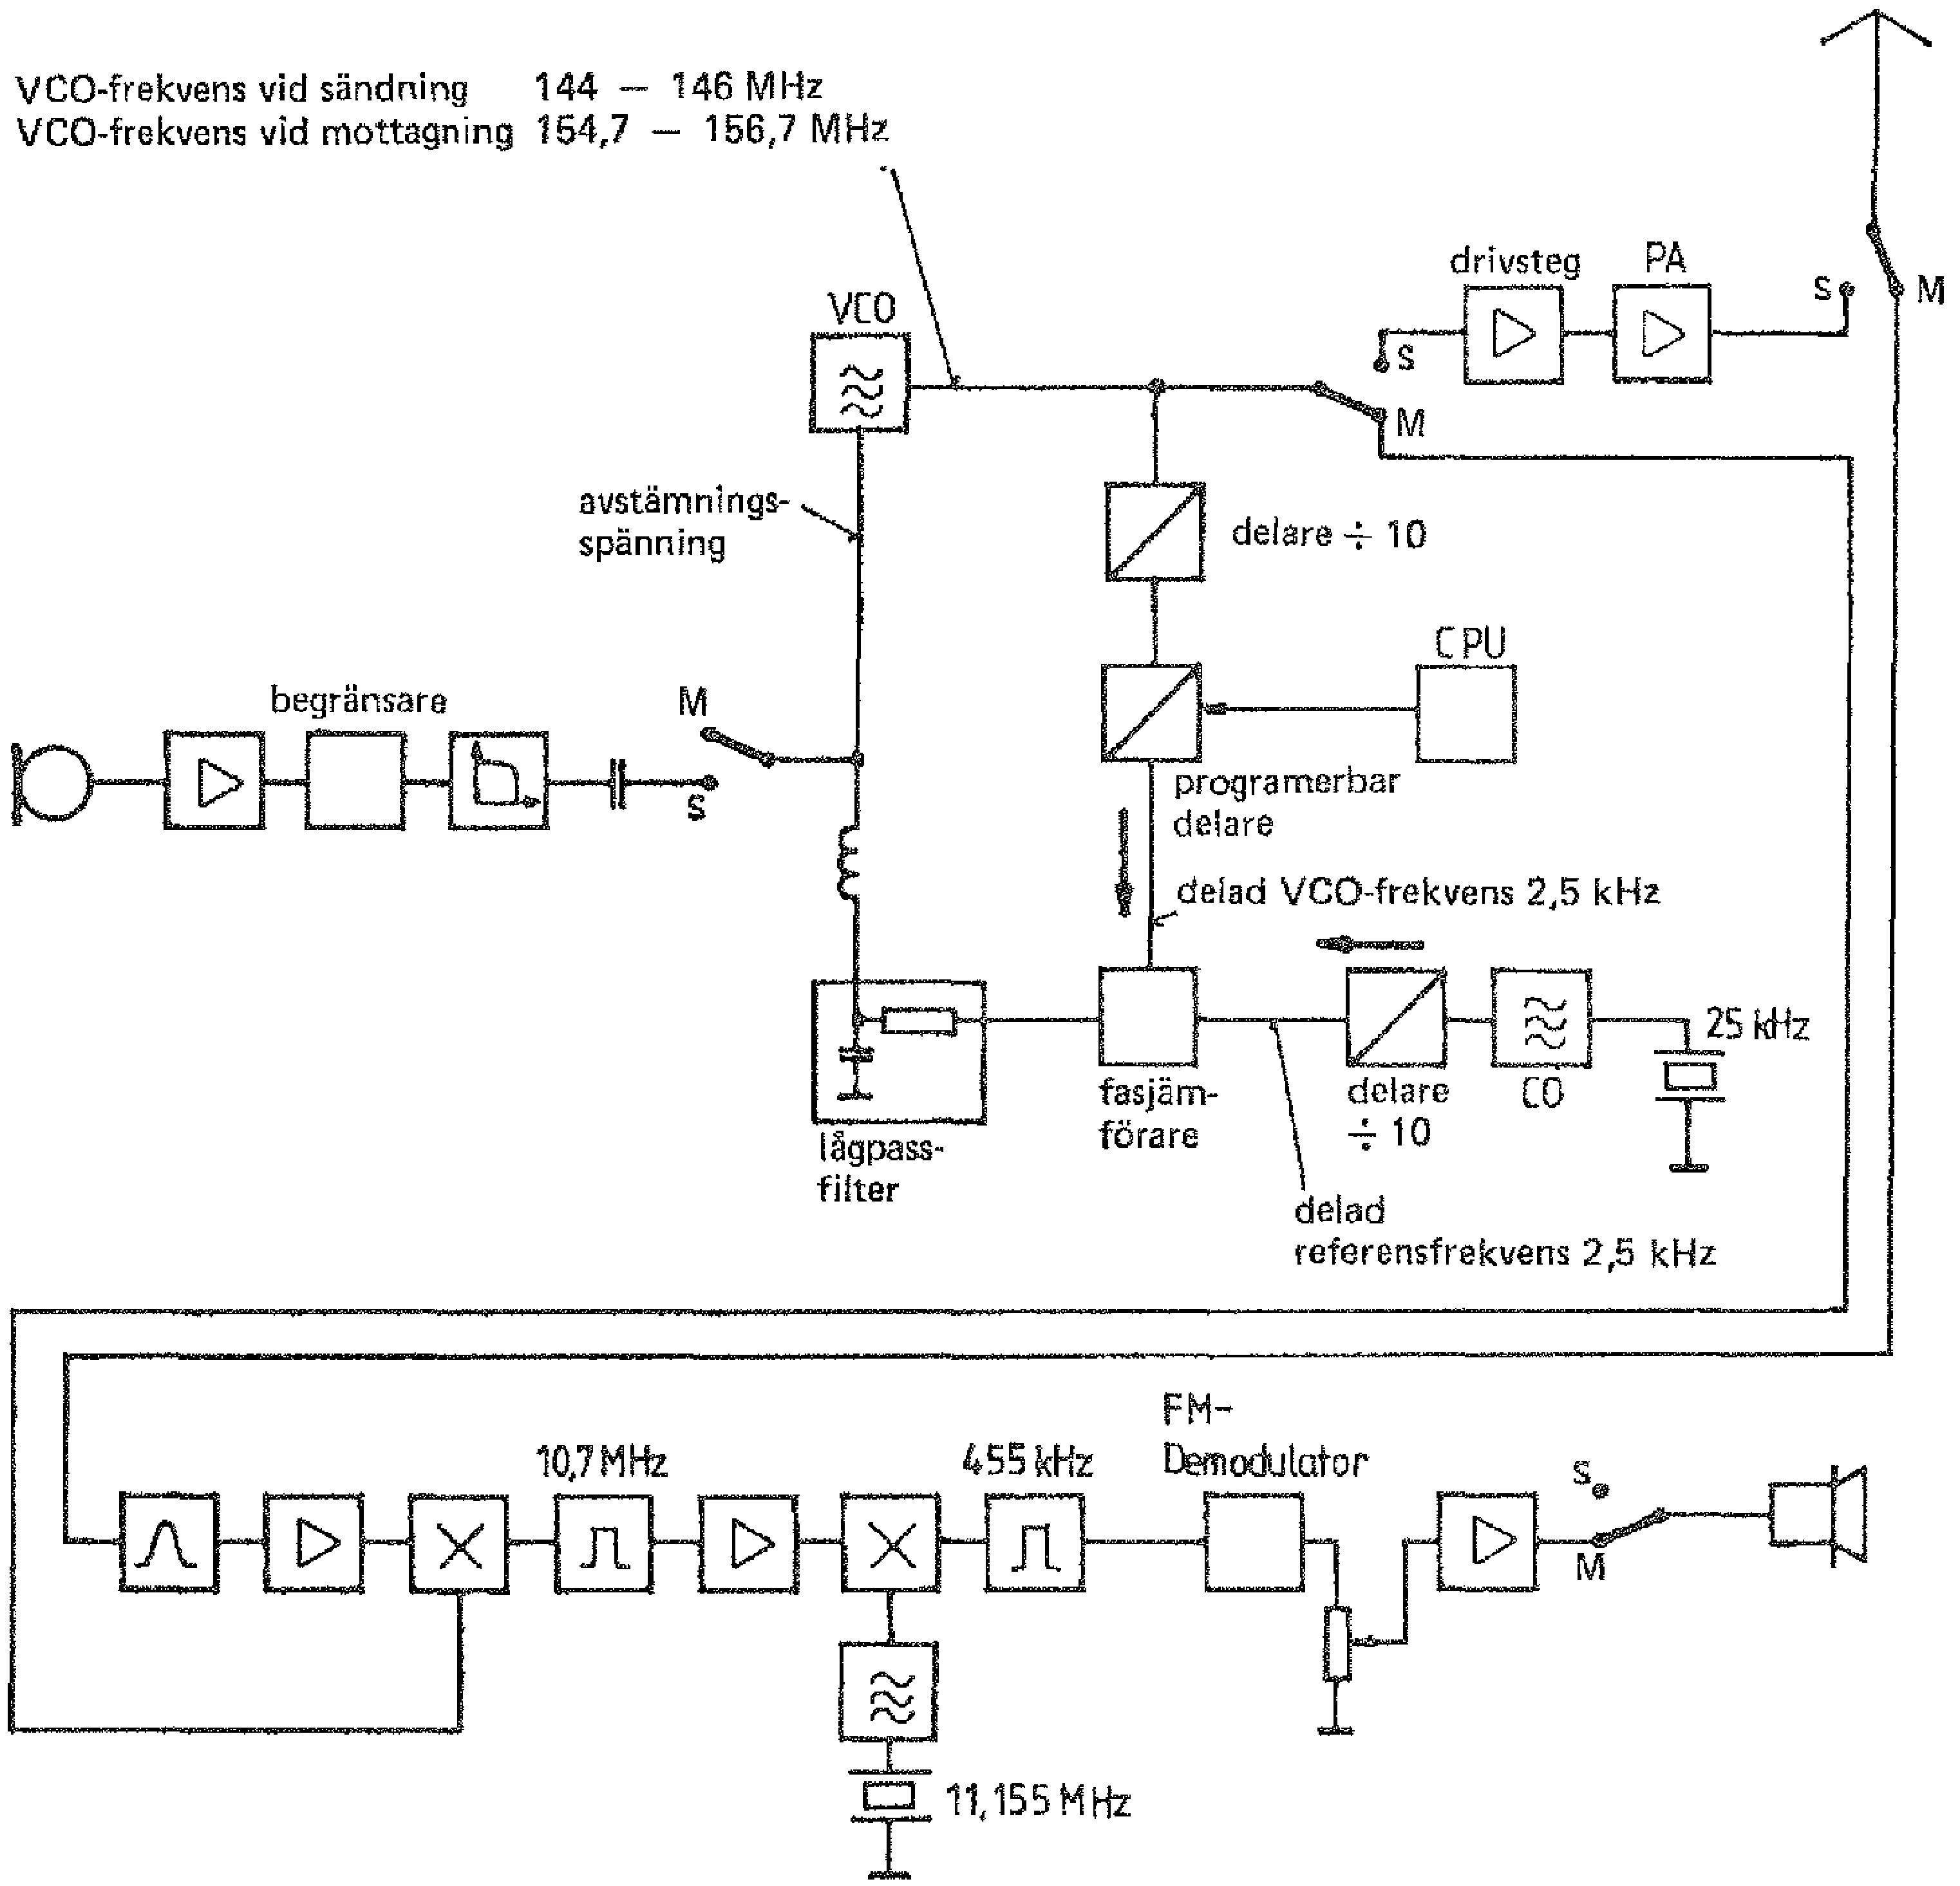
\includegraphics[width=\textwidth]{images/cropped_pdfs/bild_2_5-13.pdf}
  \caption{PLL-styrd FM-transceiver för VHF}
  \label{fig:bildII5-13}
\end{figure}

Den PLL-styrda sändare som redan beskrivits i bild \ref{fig:bildII5-7} har här
kompletterats med en svingbegränsare och ett lågpassfilter i modulatorn.
Liksom i den station med kanalkristaller, som beskrivits i
bild \ref{fig:bildII5-13}, är mottagaren även i detta fall en dubbelsuper.

VCO används även som lokaloscillator i mottagaren.
Eftersom sändaren och mottagaren ska användas på samma frekvens
(simplextrafik), måste i detta koncept VCO-frekvensen vara olika vid
sändning och mottagning.
Eftersom mottagarens mellanfrekvens MF är 10,7~MHz måste nämligen VCO
ligga 10,7~MHz högre eller lägre vid mottagning än vid sändning.
Vid sändning däremot, är VCO-frekvensen densamma som sändningsfrekvensen.

Den programmerbara frekvensdelaren i PLL-kretsen arbetar därför med
olika delningstal vid sändning respektive mottagning.
Inställningen av divisorn kan ske med kanalomkopplare, tumhjulssats,
knappsats eller ''VFO-ratt'' + digitalräknare och så vidare.
PLL-styrningen ger dessutom möjligheter, till exempel att ordna en automatisk
avsökning över ett önskat frekvensområde -- så kallad scanning.

\begin{table}[ht]
\begin{center}
  \begin{tabular}{ll|lll}
    \multicolumn{2}{l|}{Sändning} &
    \multicolumn{3}{l}{Mottagning} \\
    QRG & Deln.- & QRG & VCO & Deln.- \\
    MHZ & tal    & MHz & MHz & tal \\
    \hline
    \multicolumn{2}{l|}{Simplexkanaler,exempel} & & & \\
    144,000 & 5760 & 144,000 & 154,700 & 6188 \\
    144,025 & 5761 & 144,025 & 154,725 & 6189 \\
    & & & & \\
    \multicolumn{2}{l|}{Repeaterkanaler,exempel} & & & \\
    145,000 & 5800 & 145,600 & 156,300 & 6252 \\
    145,025 & 5801 & 145,625 & 156,325 & 6253 \\
  \end{tabular}
\end{center}
\end{table}

VCO-frekvensen är lika vid sändning och mottagning medan delningstalet
bestämmer arbetsfrekvensen.

\subsection{Kortvågstransceiver för SSB och CW}
\index{SSB}
\index{transceiver!SSB}
\index{CW}
\index{transceiver!CW}
\index{talstyrd sändning}
\index{Voice Operated Xmitter (VOX)}
\index{VOX}

Vi har redan beskrivit en KV-sändare och KV-mottagare för SSB.
I det koncept på en kortvågstransceiver, som visas här i
bild \ref{fig:bildII5-14}, ingår en super-VFO i signalberedningen.
VFO-signalen (5--5,5~MHz) blandas med signalen från en kristallstyrd CO,
vars frekvens är valbar med en bandomkopplare.
Samtidigt kopplas ett bandpassfilter in efter blandaren i super-VFO,
som svarar till det aktuella frekvensbandet.

För till exempel 21~MHz-bandet är VFO-filtrets passband 12--12,5~MHz.
När en VFO-signal 12--12,5~MHz blandas med en 9~MHz SSB modulerad signal
erhålls en frekvens i området 3--3,5~MHz och en frekvens i området 21--21,5~MHz.
Den önskade av dessa frekvenser filtreras fram med omkopplingsbara
bandpassfilter, vilket sker med den bandkopplare som nämnts tidigare.

I den enkla kortvågssändare som beskrivits tidigare är det
tillräckligt med en enda sats av omkopplingsbara bandpassfilter.
Det större antalet filter i den här beskrivna utrustningen behövs för att
även kunna använda super-VFO som en del i mottagaren, vilken arbetar
som enkelsuper.
Eftersom en MF på 9~MHz används även i mottagaren kommer mottagning och
sändning att kunna ske på samma frekvens.

Mottagaren beskrivs inte närmare.
Med lämpliga omkopplingsanordningar kan vissa funktionsblock i
transceivern användas både vid mottagning och sändning.
Bild \ref{fig:bildII5-14} visar en SSB-transceiver där passbandfilter i
förkretsar, MF-filter och kristalloscillatorer har dubbel användning.
Funktionsblocken visas inplacerade i sina alternativa
funktioner, däremot inte omkopplingsanordningarna.

Vid sändning och mottagning av CW förbikopplas den balanserade
modulatorn och kristallfiltret i signalbehandlingskretsarna för 9~MHz.
För mottagning av CW ändras BFO-frekvensen i mottagaren så att
det hörs en svävningston när en bärvåg tas emot.
Utan denna frekvensändring skulle endast bärvågsbruset höras.

Även en RIT och en \emph{talstyrd sändning} (eng.
\emph{Voice Operated Xmitter (VOX)}) är inritade.

\begin{figure}
  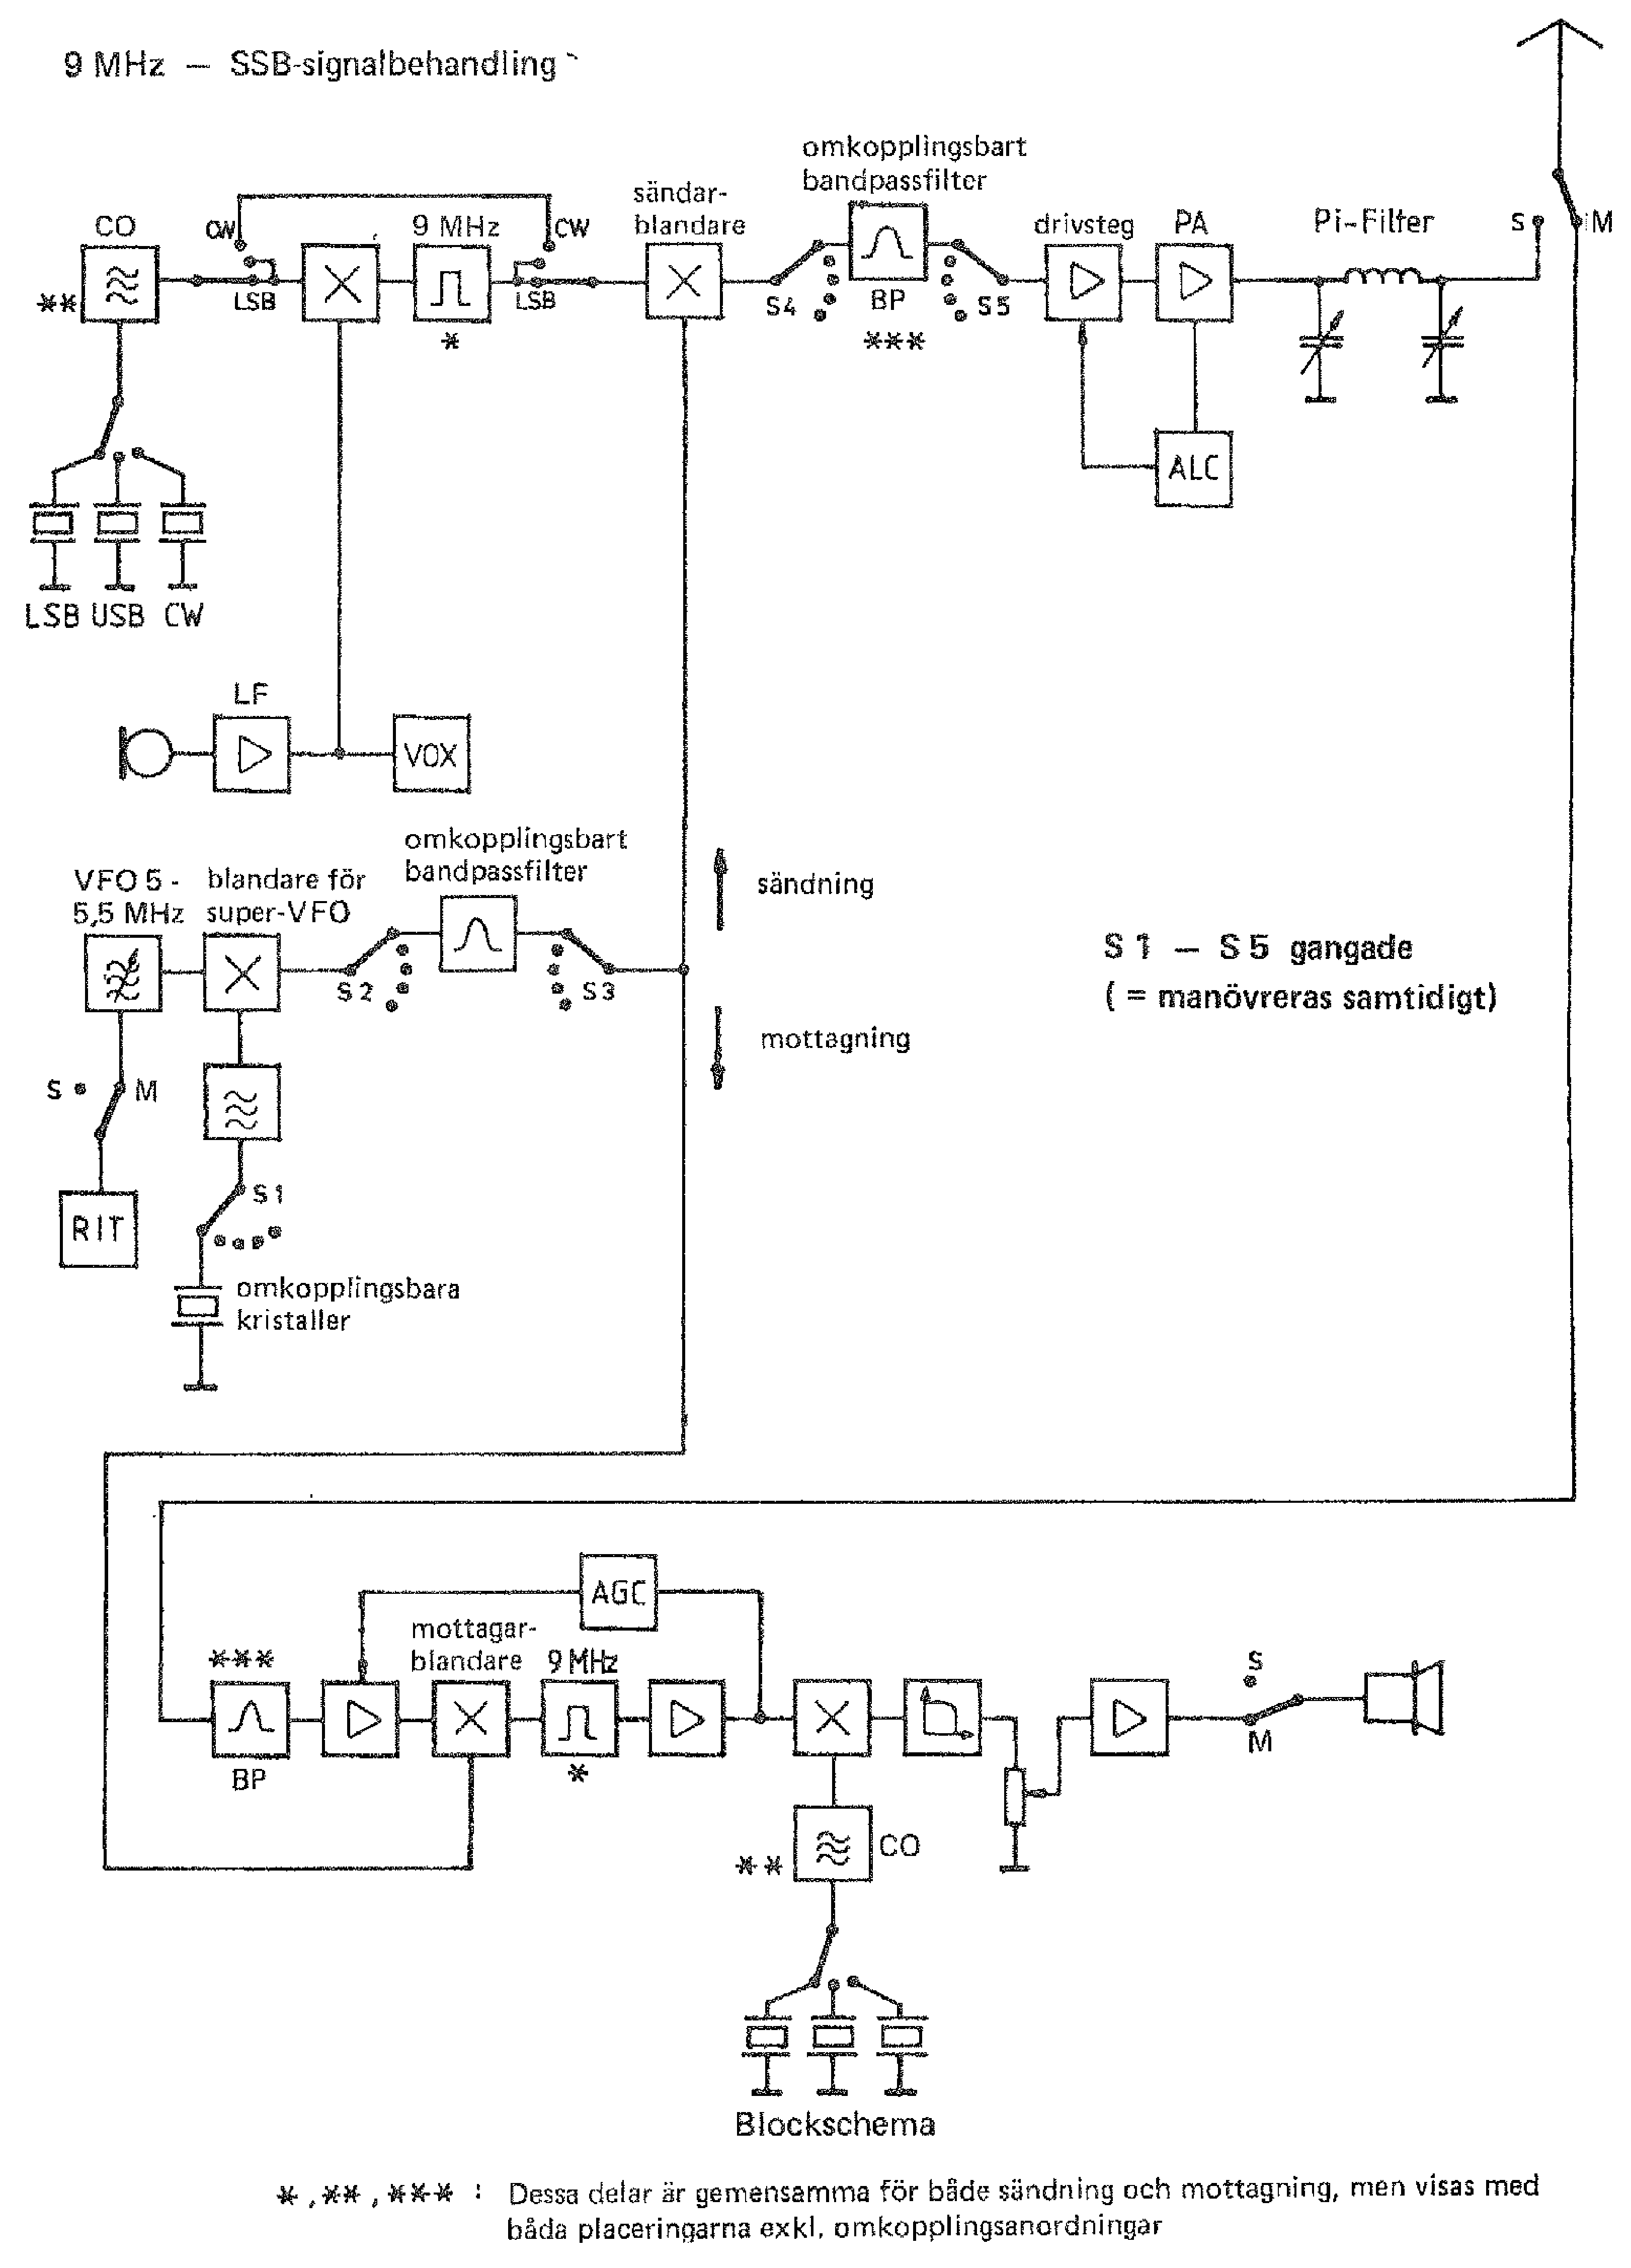
\includegraphics[width=\textwidth]{images/cropped_pdfs/bild_2_5-14.pdf}
  \caption{SSB-transceiver för kortvåg}
  \label{fig:bildII5-14}
\end{figure}

\begin{figure}
  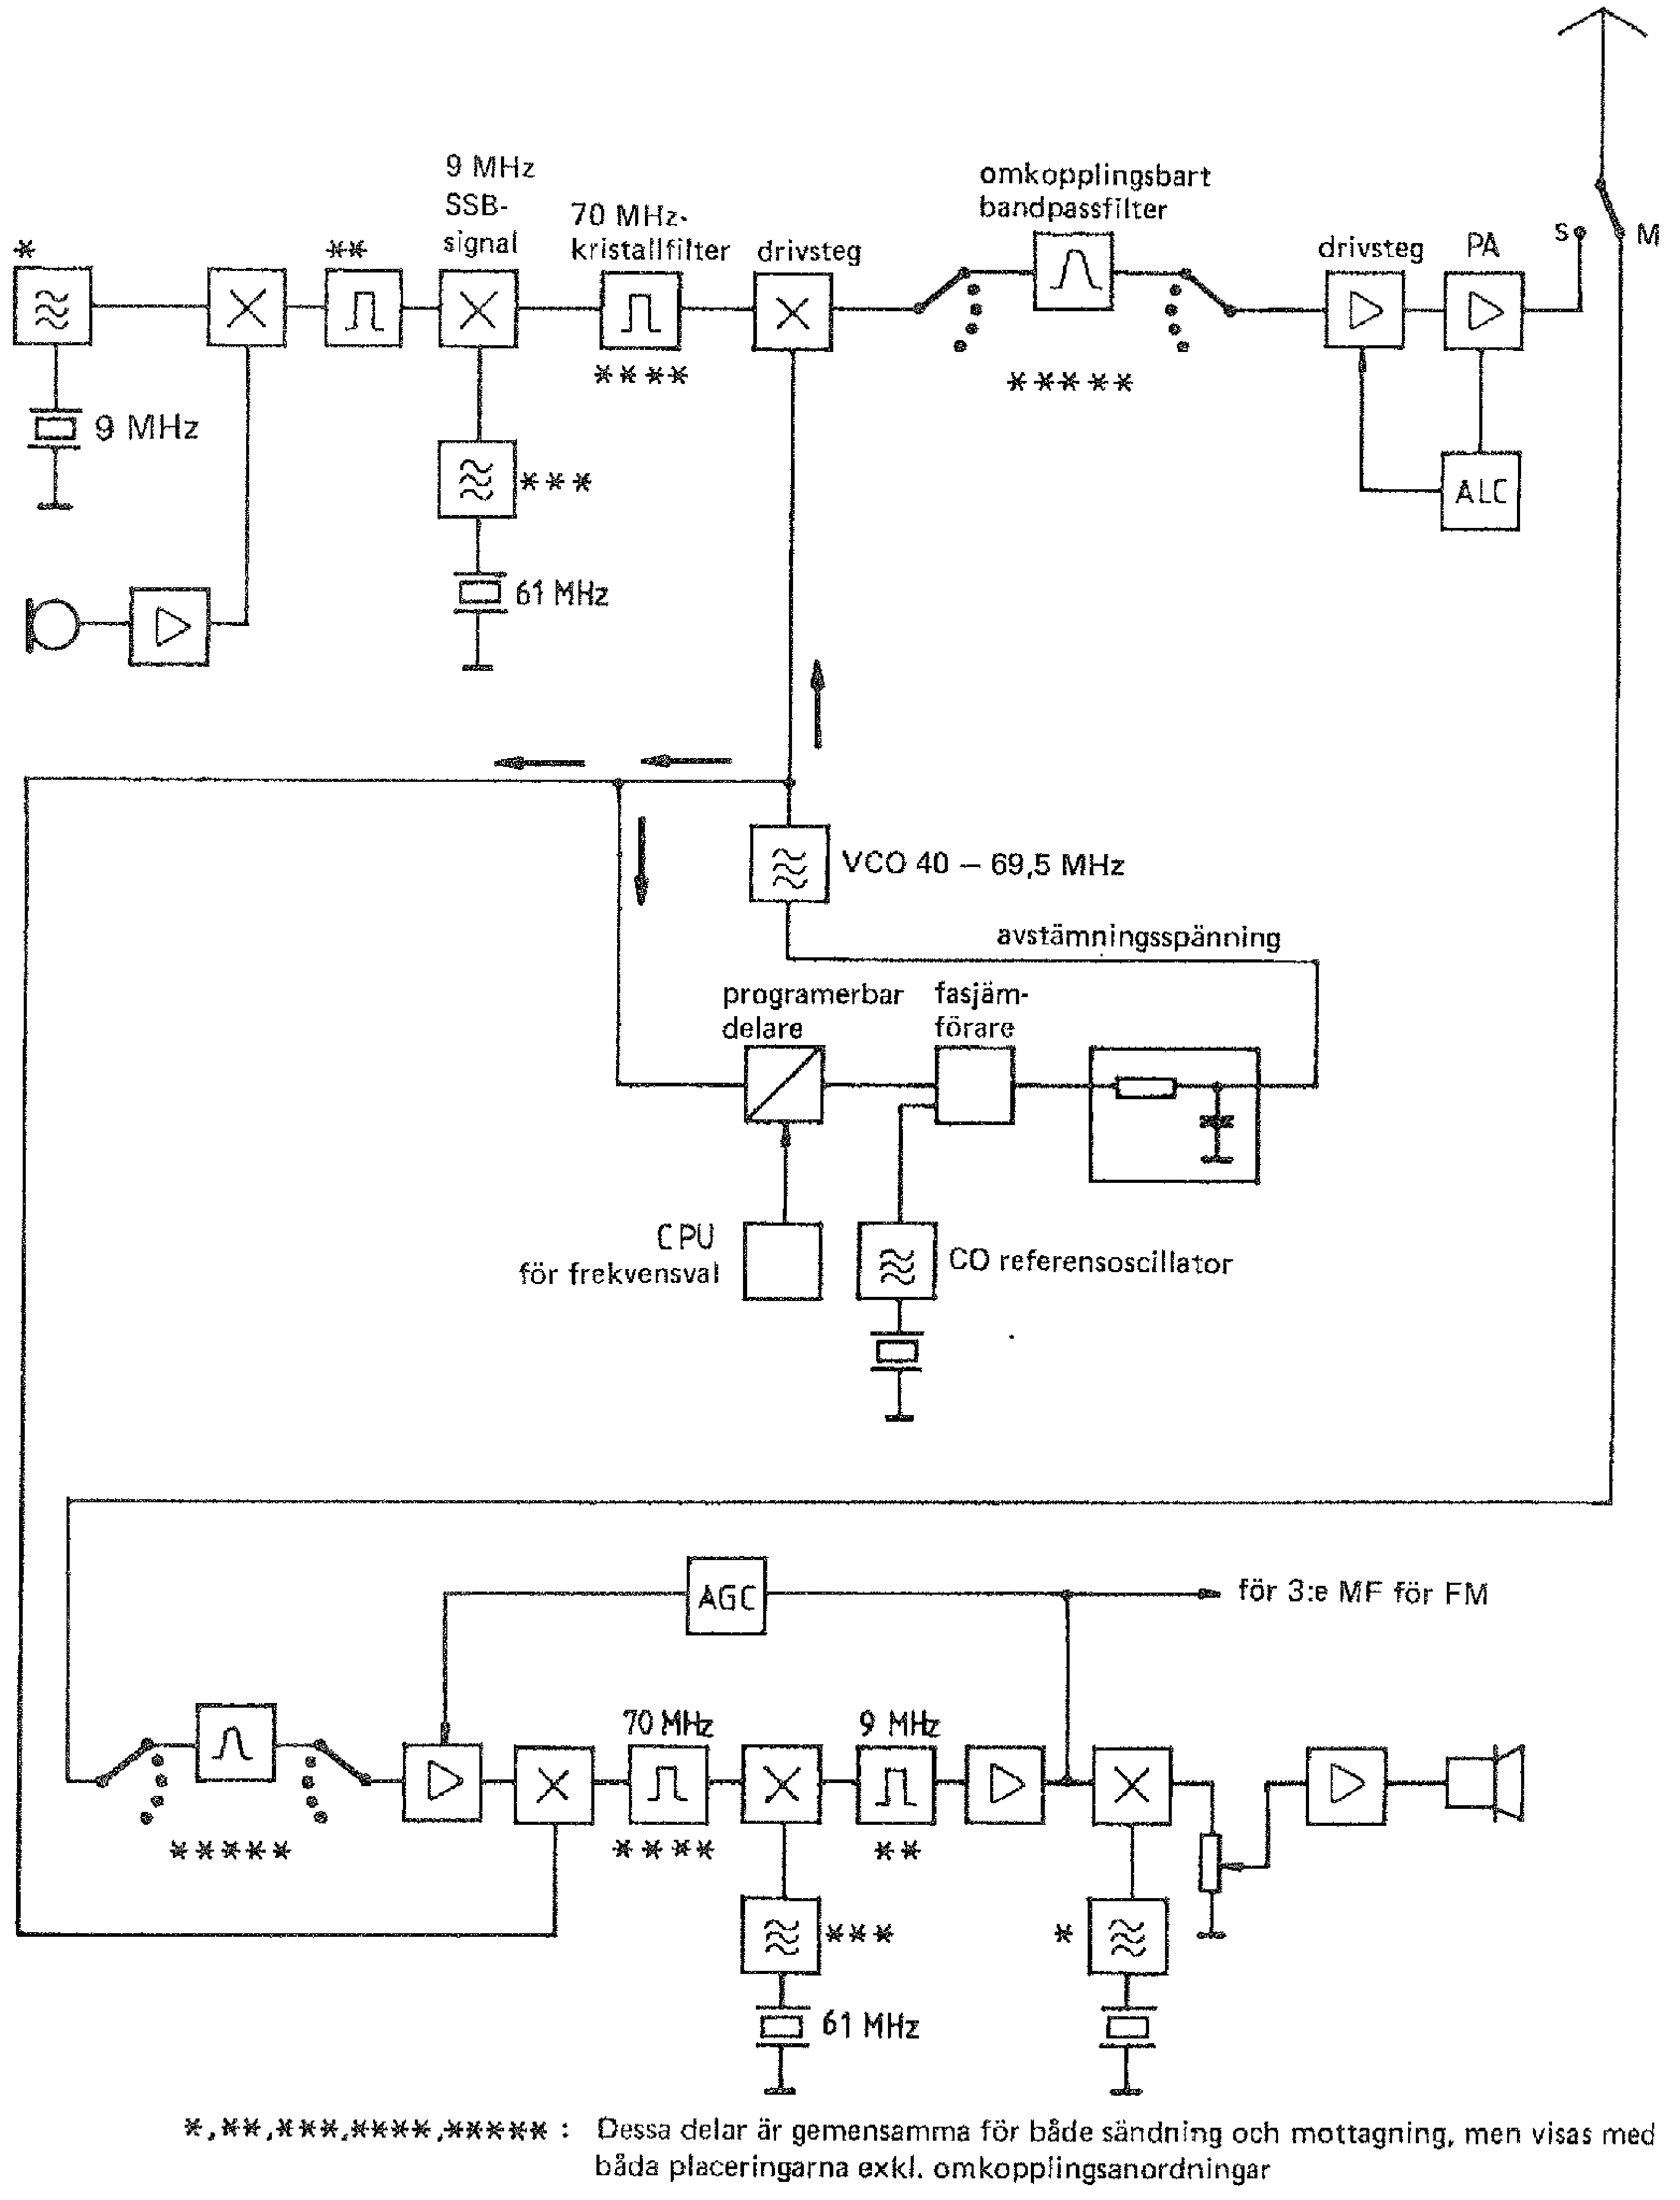
\includegraphics[width=\textwidth]{images/cropped_pdfs/bild_2_5-15.pdf}
  \caption{PLL-styrd SSB-transceiver för kortvåg}
  \label{fig:bildII5-15}
\end{figure}

\subsection{PLL-styrd kortvågstransceiver}
\index{PLL}
\index{transceiver!PLL}

En modern transceiver i den högre prisklassen finns i bild \ref{fig:bildII5-15},
i så kallad ''all-mode''-utförande, erbjuder många funktionella möjligheter.
Flera av dem kommer emellertid endast till användning i speciella situationer.
Konceptet för en sådan transceiver beskrivs här i stort.
Huvudprincipen för signalbehandlingen kan beskrivas som en PLL-styrd
dubbelsuper.
SSB-signalen bereds på 9~MHz-nivån och flyttas därefter upp till
70~MHz-nivån genom frekvensblandning och filtrering.
De möjliga sändningsfrekvenserna mellan 0,5 och 30~MHz skapas genom att
blanda den fasta SSB-signalen med en variabel frekvens från VCO.
Den steglösa frekvenstäckningen som innefattar mellanvågs- och kortvågsområdet
är emellertid endast avsedd för mottagningsfunktionen i transceivern.
För sändningsfunktionen kan tillkomma blockeringskretsar, som förhindrar
sändning utanför tillåtna frekvensband.

Denna förenklade beskrivning omfattar inte kristalloscillatorerna för
9 och 61~MHz i fasregleringskretsen och inte heller SSB-modulatorn,
FM-modulatorn och anordningarna för CW-sändning.

Mottagaren är en dubbelsuper med hög 1:a MF-frekvens.
Mottagare för höga frekvenser kan till och med utföras som en trippelsuper.
Samma bandpassfilter, blandare och kristallfilter används både vid sändning
och mottagning.

Genom lämplig programmering av frekvensdelaren kan sändning och
mottagning ske på samma frekvens eller på skilda frekvenser
(split-trafik).

En extra VFO-funktion kan åstadkommas genom att frekvensdelaren
programmeras med delningstal som hämtas från ett digitalt minne.
Den extra VFO-funktionen kan sedan efterjusteras genom att ändra
delningstalet med frekvensratten.
Minnet blir ännu mer användbart, om det förutom frekvenser också kan lagra
uppgifter till exempel om sändningsslag och andra inställningar.

\subsection{Sammanfattning}

Till skillnad från den raka sändaren är den här beskrivna PLL-styrda
transceivern mycket komplicerad.
Den tekniska utvecklingen går fort.
Nya, bättre och mer invecklade apparater utvecklas ständigt.
Men det är inte alls nödvändigt att använda det senaste och mest
avancerade inom apparattekniken för att utöva amatörradio.
Det går mycket bra att börja med enkla medel och med liten ekonomisk insats.

Det finns ett stort utbud av begagnade apparater som i olika avseenden
är konkurrenskraftiga med senare konstruktioner.
Det ligger i amatörradions traditioner att ta tillvara tillgänglig
utrustning och förbättra denna efter bästa förmåga.

Ytterst beror resultatet och framgången mest på radiooperatörens
skicklighet, val av frekvens, antenn och tillfälle.
